\documentclass[10pt,a4paper]{article}
\usepackage[a4paper,top=3.3cm,bottom=2.1cm,left=1.5cm,right=1.5cm,headheight=42pt,headsep=10pt,footskip=24pt]{geometry}
\usepackage[T1]{fontenc}
\usepackage{amsmath,amssymb}
\usepackage{xcolor}
\usepackage{tikz}
\usetikzlibrary{arrows.meta,calc,patterns}
\usepackage{fancyhdr}
\usepackage{lastpage}
\usepackage{tabularx}
\usepackage{array}
\usepackage{multicol}
\usepackage{needspace}
\usepackage{pifont}

\definecolor{spsblue}{RGB}{20,50,120}
\definecolor{spsgrey}{RGB}{110,110,110}
\setlength{\columnsep}{0.8cm}
\setlength{\columnseprule}{0.4pt}

% ---------- header / footer ----------
\pagestyle{fancy}
\fancyhf{}
\renewcommand{\headrulewidth}{0.9pt}
\renewcommand{\footrulewidth}{0.5pt}
\fancyhead[C]{%
  {\Large\bfseries\color{spsblue}SAGAR PUBLIC SCHOOL}\\[2pt]
  {\small\bfseries Integrated Programme \quad$\bullet$\quad Topic: \sheettopic}}
\fancyfoot[L]{\footnotesize Sagar Public School}
\fancyfoot[C]{\footnotesize Integrated Programme \,|\, Gravitation -- Practice Sheet \sheetno}
\fancyfoot[R]{\footnotesize Page \thepage\ of \pageref{LastPage}}
\setlength{\parindent}{0pt}
\setlength{\parskip}{0pt}
\renewcommand{\arraystretch}{1.2}

% ---------- question machinery ----------
\newcounter{qn}
\newcommand{\cursrc}{}
\newenvironment{question}[1]{%
  \par\vspace{6pt}\def\cursrc{#1}%
  \begin{minipage}{\linewidth}\refstepcounter{qn}\textbf{Q.\theqn}\quad\ignorespaces}%
 {\par\vspace{1pt}\hfill{\tiny\color{spsgrey}[\cursrc]}\end{minipage}\par}
\newcommand{\secthead}[1]{\par\vspace{8pt}\noindent\begin{minipage}{\linewidth}{\normalsize\bfseries\color{spsblue}#1}\par\vspace{1pt}\hrule height 0.6pt\end{minipage}\par\nobreak}

\newcommand{\labA}{A}\newcommand{\labB}{B}\newcommand{\labC}{C}\newcommand{\labD}{D}
\newcommand{\numlabels}{\renewcommand{\labA}{1}\renewcommand{\labB}{2}\renewcommand{\labC}{3}\renewcommand{\labD}{4}}
\newcommand{\letterlabels}{\renewcommand{\labA}{A}\renewcommand{\labB}{B}\renewcommand{\labC}{C}\renewcommand{\labD}{D}}
\newcommand{\optsfour}[4]{\par\vspace{2pt}\hspace*{1em}\begin{tabularx}{\dimexpr\linewidth-1em\relax}{*{4}{>{\raggedright\arraybackslash}X}}
 (\labA) #1 & (\labB) #2 & (\labC) #3 & (\labD) #4\end{tabularx}\par}
\newcommand{\optstwo}[4]{\par\vspace{2pt}\hspace*{1em}\begin{tabularx}{\dimexpr\linewidth-1em\relax}{*{2}{>{\raggedright\arraybackslash}X}}
 (\labA) #1 & (\labB) #2 \\ (\labC) #3 & (\labD) #4\end{tabularx}\par}
\newcommand{\optsone}[4]{\par\vspace{2pt}\begin{list}{}{\setlength{\leftmargin}{2.3em}\setlength{\labelwidth}{2em}\setlength{\itemsep}{0pt}\setlength{\topsep}{0pt}\setlength{\parsep}{0pt}}
 \item[(\labA)] #1 \item[(\labB)] #2 \item[(\labC)] #3 \item[(\labD)] #4 \end{list}\par}

\tikzset{fig/.style={line width=0.8pt,>={Stealth[length=2mm]}}}

% Motion Ex-I Q.16 : one square panel / four panels
\newcommand{\sqpanel}[6]{\begin{tikzpicture}[fig,line width=0.7pt]
 \node[left] at (-0.1,0.9) {(#1)};
 \draw (0,0) rectangle (1.8,1.8);
 \foreach \p in {(0.55,1.3),(1.25,1.3),(0.9,0.9),(0.55,0.45),(1.25,0.45)} \fill \p circle (3pt);
 \node[anchor=north west,inner sep=1pt] at (0,1.8) {\scriptsize #2};
 \node[anchor=north east,inner sep=1pt] at (1.8,1.8) {\scriptsize #3};
 \node[anchor=south west,inner sep=1pt] at (0,0) {\scriptsize #4};
 \node[anchor=south east,inner sep=1pt] at (1.8,0) {\scriptsize #5};
 \node[anchor=west,inner sep=2pt] at (0.95,0.92) {\scriptsize #6};
\end{tikzpicture}}
\newcommand{\figSquares}{\sqpanel{A}{5M}{3M}{M}{5M}{M}\hspace{0.5cm}\sqpanel{B}{2M}{3M}{M}{2M}{M}\\[6pt]
 \sqpanel{C}{5M}{3M}{M}{5M}{2M}\hspace{0.5cm}\sqpanel{D}{2M}{3M}{M}{2M}{2M}}

% JEE Main 2026 22 Jan Morning : four masses at corners
\newcommand{\figSquare}{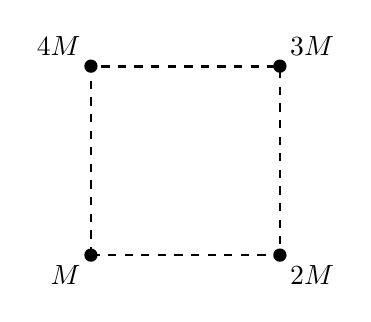
\begin{tikzpicture}[fig]
 \draw[dashed,line width=1pt] (0,0) rectangle (2.4,2.4);
 \foreach \p in {(0,0),(2.4,0),(0,2.4),(2.4,2.4)} \fill \p circle (2.4pt);
 \node[above left] at (0,2.4) {$4M$}; \node[above right] at (2.4,2.4) {$3M$};
 \node[below left] at (0,0) {$M$}; \node[below right] at (2.4,0) {$2M$};
\end{tikzpicture}}

% Motion Ex-I Q.22 : energy versus orbit radius
\newcommand{\figEnergy}{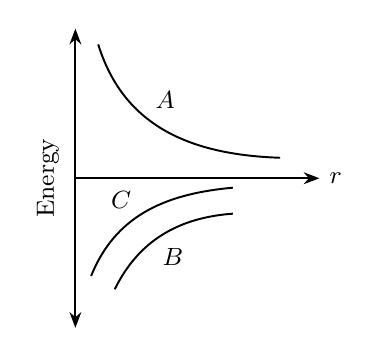
\begin{tikzpicture}[fig,line width=0.7pt]
 \draw[<->] (0,-1.9)--(0,1.9); \node[rotate=90] at (-0.35,0) {\small Energy};
 \draw[->] (0,0)--(3.1,0) node[right] {\small $r$};
 \draw (0.29,1.7) .. controls (0.6,0.7) and (1.4,0.3) .. (2.6,0.26); \node at (1.14,1.0) {\small $A$};
 \draw (0.2,-1.24) .. controls (0.5,-0.5) and (1.1,-0.2) .. (2.0,-0.12); \node at (0.58,-0.28) {\small $C$};
 \draw (0.5,-1.41) .. controls (0.8,-0.8) and (1.3,-0.5) .. (2.0,-0.45); \node at (1.24,-1.0) {\small $B$};
\end{tikzpicture}}

% Motion Ex-III Q.9 : two satellites on a collision course
\newcommand{\figOrbit}{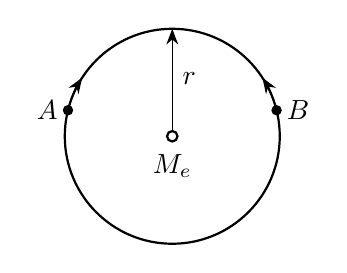
\begin{tikzpicture}[fig,scale=1.05]
 \draw (0,0) circle (1.3);
 \draw[->,line width=0.5pt] (0,0) -- (0,1.3); \node[right] at (0,0.7) {$r$};
 \draw[fill=white] (0,0) circle (1.8pt); \node[below] at (0,-0.1) {$M_e$};
 \fill (166:1.3) circle (1.8pt); \node[left] at (166:1.3) {$A$};
 \fill (14:1.3) circle (1.8pt); \node[right] at (14:1.3) {$B$};
 \draw[->,line width=0.5pt] (166:1.3) arc (166:147:1.3);
 \draw[->,line width=0.5pt] (14:1.3) arc (14:33:1.3);
\end{tikzpicture}}

% Motion Ex-III Q.15 : sphere with spherical hole
\newcommand{\figHole}{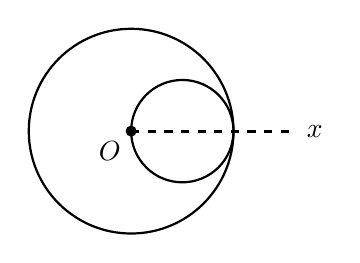
\begin{tikzpicture}[fig]
 \draw (0,0) circle (1.3); \draw (0.65,0) circle (0.65);
 \fill (0,0) circle (2pt); \node[below left] at (0,0) {$O$};
 \draw[dashed,line width=1pt] (0,0)--(2.1,0); \node[right] at (2.1,0) {$x$};
\end{tikzpicture}}

% Motion Ex-IV Q.3 : infinite rod with lambda(x) = lambda / x
\newcommand{\figInfRod}{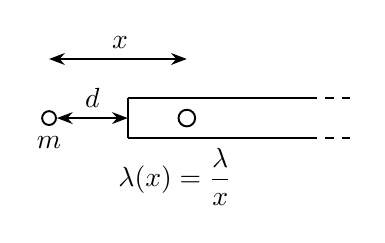
\begin{tikzpicture}[fig,line width=0.7pt]
 \draw (0,0) circle (2.5pt); \node[below] at (0,-0.1) {$m$};
 \draw[<->] (0.1,0)--(1.0,0); \node[above] at (0.55,0) {$d$};
 \draw (1.0,-0.25)--(1.0,0.25); \draw (1.0,0.25)--(3.3,0.25); \draw (1.0,-0.25)--(3.3,-0.25);
 \draw[dashed] (3.3,0.25)--(3.9,0.25); \draw[dashed] (3.3,-0.25)--(3.9,-0.25);
 \draw[fill=white] (1.75,0) circle (3pt);
 \draw[<->] (0,0.75)--(1.75,0.75); \node[above] at (0.9,0.75) {$x$};
 \node at (1.6,-0.75) {$\lambda(x)=\dfrac{\lambda}{x}$};
\end{tikzpicture}}

% Nucleus JM Q.10 (JEE Main 2017) : g versus d
\newcommand{\gpanel}[2]{\begin{tikzpicture}[fig,line width=0.7pt,scale=0.85]
 \draw[->] (0,0)--(2.4,0) node[right] {\scriptsize $d$}; \draw[->] (0,0)--(0,1.8) node[above] {\scriptsize $g$};
 \node[below left] at (0,0) {\scriptsize $O$}; \node[left] at (-0.25,0.9) {(#1)};
 #2
\end{tikzpicture}}
\newcommand{\figGraphs}{%
 \gpanel{1}{\draw (0,0) .. controls (0.9,0) and (1.5,0.3) .. (1.95,1.6);}\hspace{0.6cm}
 \gpanel{2}{\draw (0,0) .. controls (0.6,0.05) and (0.95,0.5) .. (1.1,1.5) .. controls (1.25,0.5) and (1.7,0.08) .. (2.2,0.02);
  \draw[dotted] (1.1,0)--(1.1,1.5); \node[below] at (1.1,0) {\scriptsize $R$};}\\[6pt]
 \gpanel{3}{\draw (0,0) .. controls (0.6,0.05) and (0.95,0.5) .. (1.1,1.5) -- (1.85,0);
  \draw[dotted] (1.1,0)--(1.1,1.5); \node[below] at (1.1,0) {\scriptsize $R$};}\hspace{0.6cm}
 \gpanel{4}{\draw (0,0)--(1.1,1.5) .. controls (1.25,0.5) and (1.7,0.08) .. (2.2,0.02);
  \draw[dotted] (1.1,0)--(1.1,1.5); \node[below] at (1.1,0) {\scriptsize $R$};}}

% Nucleus JM Q.8 (JEE Main 2015) : sphere with cavity
\newcommand{\figCavityHatch}{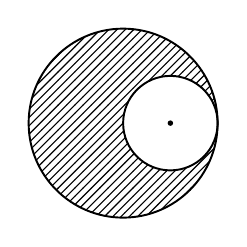
\begin{tikzpicture}[fig,line width=0.7pt]
 \path[pattern=north east lines,even odd rule] (0,0) circle (1.2) (0.6,0) circle (0.6);
 \draw (0,0) circle (1.2); \draw (0.6,0) circle (0.6); \fill (0.6,0) circle (1pt);
\end{tikzpicture}}

% Nucleus JM Q.35 (JEE Main 2021) : two satellites
\newcommand{\figTwoSat}{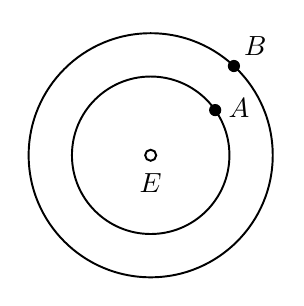
\begin{tikzpicture}[fig,line width=0.7pt]
 \draw (0,0) circle (1.0); \draw (0,0) circle (1.55);
 \draw[fill=white] (0,0) circle (2pt); \node[below] at (0,-0.1) {$E$};
 \fill (35:1.0) circle (2.2pt); \node[right] at (35:1.05) {$A$};
 \fill (47:1.55) circle (2.2pt); \node[above right] at (47:1.55) {$B$};
\end{tikzpicture}}

% JEE Main 2025 22 Jan Morning : sphere with spherical part removed
\newcommand{\figHoleP}{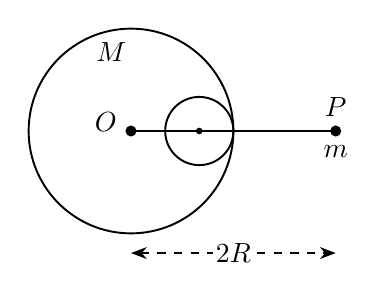
\begin{tikzpicture}[fig,line width=0.7pt]
 \draw (0,0) circle (1.3); \draw (0.867,0) circle (0.433);
 \fill (0,0) circle (2pt); \node[left] at (-0.05,0.12) {$O$};
 \fill (0.867,0) circle (1.2pt);
 \draw (0,0)--(2.6,0); \fill (2.6,0) circle (2pt);
 \node[above] at (2.6,0.05) {$P$}; \node[below] at (2.6,-0.05) {$m$};
 \node at (-0.25,1.0) {$M$};
 \draw[<->,dashed] (0,-1.55)--(2.6,-1.55); \node[fill=white,inner sep=1pt] at (1.3,-1.55) {$2R$};
\end{tikzpicture}}

% ---------- title block, answer key items, self assessment ----------
\newcommand{\titleblock}[2]{%
 \begin{center}
  {\Large\bfseries PRACTICE SHEET -- \sheetno}\\[2pt]
  {\normalsize\bfseries #1}
 \end{center}
 \vspace{1pt}
 \noindent\begin{tabularx}{\linewidth}{|X|X|X|}\hline
  Name: \hrulefill & Class / Section: \hrulefill & Date: \hrulefill \\ \hline
  \textbf{Time Allowed: 60 Mins} & \textbf{Total Questions: #2} & Roll No.: \hrulefill \\ \hline
 \end{tabularx}
 \par\vspace{4pt}}
\newcommand{\keyitem}[3]{\par\noindent\begin{minipage}{\linewidth}\textbf{#1.} {\scriptsize\color{spsgrey}[#2]}\ \ #3\end{minipage}\par\vspace{5pt}}

\newcommand{\selfassess}{%
 \clearpage
 \begin{center}{\Large\bfseries SELF ASSESSMENT -- Practice Sheet \sheetno}\end{center}
 \noindent\textit{Fill this in after checking your answers with the Answer Key.}\par\vspace{6pt}
 \noindent\begin{tabularx}{\linewidth}{|X|X|}\hline
  \textbf{Time Allowed:} 60 Mins & \textbf{Time Taken:} \rule{2.2cm}{0.4pt} Mins \\ \hline
  Start time: \rule{2cm}{0.4pt} & End time: \rule{2cm}{0.4pt} \\ \hline
  \multicolumn{2}{|l|}{Finished within the allowed time?\quad $\square$ Yes \quad $\square$ No \quad (extra / saved time: \rule{1.6cm}{0.4pt} Mins)} \\ \hline
 \end{tabularx}
 \par\vspace{8pt}
 \noindent\begin{tabularx}{\linewidth}{|>{\centering\arraybackslash}X|>{\centering\arraybackslash}X|>{\centering\arraybackslash}X|>{\centering\arraybackslash}X|>{\centering\arraybackslash}X|}\hline
  \textbf{Total} & \textbf{Attempted} & \textbf{Correct} & \textbf{Incorrect} & \textbf{Not attempted} \\ \hline
  15 & \rule[-4pt]{0pt}{18pt} & & & \\ \hline
 \end{tabularx}
 \par\vspace{3pt}
 \noindent Score (Correct $/$ 15): \rule{1.8cm}{0.4pt} \qquad Percentage: \rule{1.8cm}{0.4pt}\,\%
 \par\vspace{8pt}
 \noindent\textbf{Question-wise tracker} \hfill {\footnotesize write \ding{51} (correct), \ding{55} (incorrect) or $-$ (not attempted)}\par\vspace{3pt}
 \noindent\begin{tabularx}{\linewidth}{|*{8}{>{\centering\arraybackslash}X|}}\hline
  1&2&3&4&5&6&7&8\\ \hline \rule[-5pt]{0pt}{18pt}&&&&&&&\\ \hline
  9&10&11&12&13&14&15& \\ \hline \rule[-5pt]{0pt}{18pt}&&&&&&&\\ \hline
 \end{tabularx}
 \par\vspace{8pt}
 \noindent\textbf{Reason for the incorrect / unattempted questions} (write question numbers)\par\vspace{2pt}
 \noindent\begin{tabularx}{\linewidth}{|X|X|}\hline
  Concept not clear: \hrulefill & Formula forgotten: \hrulefill \\ \hline
  Calculation / silly mistake: \hrulefill & Ran out of time: \hrulefill \\ \hline
 \end{tabularx}
 \par\vspace{8pt}
 \noindent\textbf{Personal feedback guide (tick the band that matches your score)}\par\vspace{2pt}
 \noindent\begin{tabularx}{\linewidth}{|c|c|X|}\hline
  & \textbf{Correct} & \textbf{What to do next} \\ \hline
  $\square$ & 14--15 & Excellent. Concept and speed are both strong. Move to harder JEE-level problems and keep revising formulae once a week. \\ \hline
  $\square$ & 11--13 & Good. Re-do every incorrect question without looking at the solution, then note the formula or idea you missed. \\ \hline
  $\square$ & 7--10 & Fair. Revise the theory of escape speed, orbital speed, energies of a satellite and Kepler's laws, then re-attempt this sheet after 3 days. \\ \hline
  $\square$ & 0--6 & Needs attention. Re-read the chapter notes and solved examples first, then attempt this sheet again in two parts of 30 mins. \\ \hline
 \end{tabularx}
 \par\vspace{8pt}
 \noindent\textbf{My personal feedback / action plan:}\par\vspace{4pt}
 \noindent\rule{\linewidth}{0.4pt}\par\vspace{9pt}\noindent\rule{\linewidth}{0.4pt}\par\vspace{9pt}\noindent\rule{\linewidth}{0.4pt}\par\vspace{9pt}\noindent\rule{\linewidth}{0.4pt}
 \par\vspace{10pt}
 \noindent\textbf{Teacher's remarks:}\par\vspace{4pt}
 \noindent\rule{\linewidth}{0.4pt}\par\vspace{9pt}\noindent\rule{\linewidth}{0.4pt}
 \par\vspace{14pt}
 \noindent Student's signature: \rule{4cm}{0.4pt} \hfill Teacher's signature: \rule{4cm}{0.4pt}}
\newcommand{\sheetno}{2}
\newcommand{\sheettopic}{Gravitation -- Level 2 (JEE Main Standard)}
\begin{document}
\titleblock{Gravitation -- Level 2 (JEE Main Standard): Practice Sheet 2 of 3}{15}
\noindent\textbf{Instructions:} Attempt all 15 questions; each has only one correct option. Sections: A -- Acceleration due to Gravity, B -- Gravitational Potential and Potential Energy, C -- Motion of Satellite, D -- Newton's Law, Gravitational Field and Kepler's Laws. Time Allowed: 60 Mins.

\begin{multicols}{2}
\letterlabels
\secthead{Section A -- Acceleration due to Gravity}

\begin{question}{JEE Main 2026, 5th April Morning Shift}
When one moves from a point 16 km below the earth's surface to a point 16 km above the earth's surface, the change in $g$ is approximately $\alpha\%$. The value of $\alpha$ is \underline{\hspace{1cm}}. (Take radius of the earth $=6400$ km.)
\optstwo{0.12}{0.25}{0.50}{0.75}
\end{question}

\begin{question}{JEE Main 2026, 4th April Evening Shift}
The height in terms of radius of the earth ($R$), at which the acceleration due to gravity becomes $\dfrac g9$, where $g$ is acceleration due to gravity on earth's surface, is \underline{\hspace{1cm}}.
\optstwo{$\sqrt3R$}{$2\sqrt2R$}{$2R$}{$\dfrac49R$}
\end{question}

\begin{question}{Motion, Ex-I Q.3}
Let $\omega$ be the angular velocity of the earth's rotation about its axis. Assume that the acceleration due to gravity on the earth's surface has the same value at the equator and the poles. An object weighed at the equator gives the same reading as a reading taken at a depth $d$ below earth's surface at a pole ($d\ll R$). The value of $d$ is
\optstwo{$\dfrac{\omega^2R^2}{g}$}{$\dfrac{\omega^2R^2}{2g}$}{$\dfrac{2\omega^2R^2}{g}$}{$\dfrac{\sqrt{Rg}}{g}$}
\end{question}

\numlabels
\begin{question}{Nucleus, JM Q.26 \; [JEE Main-2020]}
The value of the acceleration due to gravity is $g_1$ at a height $h=\dfrac R2$ ($R$ = radius of the earth) from the surface of the earth. It is again equal to $g_1$ at a depth $d$ below the surface of the earth. The ratio $\left(\dfrac dR\right)$ equals:
\optstwo{$\dfrac13$}{$\dfrac59$}{$\dfrac49$}{$\dfrac79$}
\end{question}

\letterlabels
\secthead{Section B -- Gravitational Potential and Potential Energy}

\begin{question}{JEE Main 2026, 5th April Evening Shift}
A body of mass $m$ is taken from the surface of earth to a height equal to twice the radius of earth ($R_e$). The increase in potential energy will be \underline{\hspace{1cm}}. ($g$ is acceleration due to gravity at the surface of earth)
\optstwo{$\dfrac12 mgR_e$}{$\dfrac34 mgR_e$}{$\dfrac14 mgR_e$}{$\dfrac23 mgR_e$}
\end{question}

\begin{question}{JEE Main 2026, 2nd April Evening Shift}
If a body of mass 1 kg falls on the earth from infinity, it attains velocity ($v$) and kinetic energy ($k$) on reaching the surface of earth. The values of $v$ and $k$ respectively are \underline{\hspace{1cm}}. (Take radius of earth to be 6400 km and $g=9.8$ m/s$^2$)
\optsone{11.2 km/s; $6.27\times10^{7}$ J}
{11.2 km/s; $12.54\times10^{7}$ J}
{8.8 km/s; $6.27\times10^{7}$ J}
{8.8 km/s; $12.54\times10^{7}$ J}
\end{question}

\begin{question}{JEE Main 2025, 4th April Evening Shift}
An object is kept at rest at a distance of $3R$ above the earth's surface where $R$ is earth's radius. The minimum speed with which it must be projected so that it does not return to earth is: (Assume mass of earth $M$, $G=$ Universal gravitational constant)
\optstwo{$\sqrt{\dfrac{3GM}{R}}$}{$\sqrt{\dfrac{2GM}{R}}$}{$\sqrt{\dfrac{GM}{2R}}$}{$\sqrt{\dfrac{GM}{R}}$}
\end{question}

\numlabels
\begin{question}{Nucleus, JM Q.3 \; [AIEEE-2011]}
Two bodies of masses $m$ and $4m$ are placed at a distance $r$. The gravitational potential at a point on the line joining them where the gravitational field is zero is:
\optstwo{zero}{$-\dfrac{4Gm}{r}$}{$-\dfrac{6Gm}{r}$}{$-\dfrac{9Gm}{r}$}
\end{question}

\letterlabels
\secthead{Section C -- Motion of Satellite}

\begin{question}{JEE Main 2024, 8th April Evening Shift}
Two satellite $A$ and $B$ go round a planet in circular orbits having radii $4R$ and $R$ respectively. If the speed of $A$ is $3v$, the speed of $B$ will be:
\optstwo{$6v$}{$\dfrac43v$}{$3v$}{$12v$}
\end{question}

\begin{question}{JEE Main 2024, 5th April Evening Shift}
A satellite revolving around a planet in stationary orbit has time period 6 hours. The mass of planet is one-fourth the mass of earth. The radius of orbit of the satellite is: (Given $=$ Radius of geo-stationary orbit for earth is $4.2\times10^4$ km)
\optstwo{$1.68\times10^5$ km}{$1.4\times10^4$ km}{$8.4\times10^4$ km}{$1.05\times10^4$ km}
\end{question}

\begin{question}{JEE Main 2026, 21st January Morning Shift}
Initially a satellite of 100 kg is in a circular orbit of radius $1.5R_E$. This satellite can be moved to a circular orbit of radius $3R_E$ by supplying $\alpha\times10^{6}$ J of energy. The value of $\alpha$ is \underline{\hspace{1cm}}. (Take Radius of Earth $R_E=6\times10^{6}$ m and $g=10$ m/s$^2$)
\optstwo{500}{1000}{100}{150}
\end{question}

\secthead{Section D -- Newton's Law, Gravitational Field and Kepler's Laws}

\begin{question}{Motion, Ex-I Q.5}
A man of mass $m$ starts falling towards a planet of mass $M$ and radius $R$. As he reaches near to the surface, he realizes that he will pass through a small hole in the planet. As he enters the hole, he sees that the planet is really made of two pieces a spherical shell of negligible thickness of mass $2M/3$ and a point mass $M/3$ at the centre. Change in the force of gravity experienced by the man is
\optstwo{$\dfrac23\dfrac{GMm}{R^2}$}{$0$}{$\dfrac13\dfrac{GMm}{R^2}$}{$\dfrac43\dfrac{GMm}{R^2}$}
\end{question}

\numlabels
\begin{question}{Nucleus, JM Q.16 \; [JEE Main-2019]}
A solid sphere of mass $M$ and radius $a$ is surrounded by a uniform concentric spherical shell of thickness $2a$ and mass $2M$. The gravitational field at distance $3a$ from the centre will be:
\optstwo{$\dfrac{GM}{3a^2}$}{$\dfrac{2GM}{9a^2}$}{$\dfrac{GM}{9a^2}$}{$\dfrac{2GM}{3a^2}$}
\end{question}

\letterlabels
\begin{question}{JEE Main 2026, 22nd January Morning Shift}
Net gravitational force at the center of a square is found to be $F_1$ when four particles having mass $M$, $2M$, $3M$ and $4M$ are placed at the four corners of the square as shown in figure and it is $F_2$ when the positions of $3M$ and $4M$ are interchanged. The ratio $\dfrac{F_1}{F_2}$ is $\dfrac{\alpha}{\sqrt5}$. The value of $\alpha$ is \underline{\hspace{1cm}}.
\begin{center}\figSquare\end{center}
\optstwo{2}{$2\sqrt5$}{1}{3}
\end{question}

\numlabels
\begin{question}{Nucleus, JM Q.31 \; [JEE Main-2021]}
Two stars of masses $m$ and $2m$ at a distance $d$ rotate about their common centre of mass in free space. The period of revolution is:
\optstwo{$\dfrac{1}{2\pi}\sqrt{\dfrac{d^3}{3Gm}}$}{$2\pi\sqrt{\dfrac{d^3}{3Gm}}$}{$\dfrac{1}{2\pi}\sqrt{\dfrac{3Gm}{d^3}}$}{$2\pi\sqrt{\dfrac{3Gm}{d^3}}$}
\end{question}
\end{multicols}

%==================== ANSWER KEY ====================
\clearpage
\begin{center}{\Large\bfseries ANSWER KEY -- Practice Sheet \sheetno}\end{center}
\noindent{\small Answers are taken from the source answer keys: Motion (Answer Ex-I), Nucleus (Answer Key page; JM answers are option numbers) and the JEE PYQ file (Answer Key at the end).}\par\vspace{4pt}
\begin{multicols}{2}
\keyitem{1}{JEE PYQ file Q.2}{B}
\keyitem{2}{JEE PYQ file Q.3}{C}
\keyitem{3}{Motion Ex-I Q.3}{A}
\keyitem{4}{Nucleus JM Q.26}{(2)}
\keyitem{5}{JEE PYQ file Q.1}{D}
\keyitem{6}{JEE PYQ file Q.4}{A}
\keyitem{7}{JEE PYQ file Q.12}{C}
\keyitem{8}{Nucleus JM Q.3}{(4)}
\keyitem{9}{JEE PYQ file Q.20}{A}
\keyitem{10}{JEE PYQ file Q.24}{D}
\keyitem{11}{JEE PYQ file Q.10}{B}
\keyitem{12}{Motion Ex-I Q.5}{A}
\keyitem{13}{Nucleus JM Q.16}{(1)}
\keyitem{14}{JEE PYQ file Q.9}{A}
\keyitem{15}{Nucleus JM Q.31}{(2)}
\end{multicols}

\selfassess
\end{document}
